% The BLAKE2 work vector [RFC 7693, §3.2]: v[0..7] = h, v[8..15] = IV, with the offset counter
% t XORed into v[12], v[13] and the final flag inverting v[14]. A round applies G to the four
% columns, then to the four diagonals.
% Original drawing for the Hash library.
\documentclass[tikz,border=6pt]{standalone}
\usepackage[T1]{fontenc}
\usepackage{lmodern}
% Shared style for the Hash diagrams.
% Palette: Okabe–Ito (colour-blind safe). Every diagram is drawn on an opaque white card so it
% stays legible on dark page themes.
\usetikzlibrary{arrows.meta,positioning,calc,fit,backgrounds}
\definecolor{hsblue}{HTML}{0072B2}
\definecolor{hsorange}{HTML}{E69F00}
\definecolor{hsgreen}{HTML}{009E73}
\definecolor{hsvermilion}{HTML}{D55E00}
\definecolor{hspurple}{HTML}{CC79A7}
\definecolor{hsink}{HTML}{1F2933}
\tikzset{
  >={Stealth[length=2.2mm]},
  every node/.style={font=\sffamily\small, text=hsink},
  wire/.style={draw=hsink, line width=0.6pt, ->},
  reg/.style={draw=hsink, line width=0.6pt, fill=hsblue!12, minimum width=9mm, minimum height=7mm},
  fn/.style={draw=hsink, line width=0.6pt, fill=hsorange!25, rounded corners=2pt, minimum width=10mm, minimum height=6mm},
  input/.style={draw=hsink, line width=0.6pt, fill=hsgreen!20, minimum width=9mm, minimum height=6mm},
  add/.style={circle, draw=hsink, line width=0.6pt, fill=white, inner sep=0pt, minimum size=5mm, font=\sffamily\bfseries},
  card/.style={fill=white, rounded corners=4pt},
}

\begin{document}
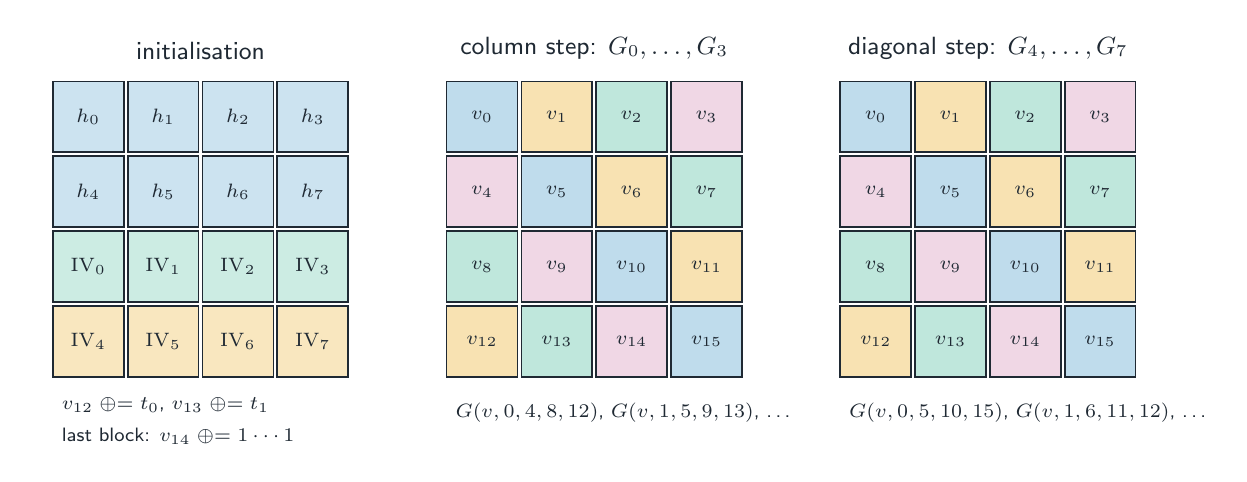
\begin{tikzpicture}[cell/.style={draw=hsink, line width=0.6pt, minimum size=9mm, inner sep=0pt,
    font=\sffamily\scriptsize, align=center}]
  \def\s{0.95}
  % Initialisation.
  \foreach \r in {0,...,3} \foreach \c in {0,...,3} {
    \pgfmathtruncatemacro{\i}{4*\r+\c}
    \ifnum\r<2 \def\col{hsblue!20}\def\lbl{$h_{\i}$}
    \else\ifnum\r=2 \def\col{hsgreen!20}\pgfmathtruncatemacro{\j}{\i-8}\def\lbl{$\mathrm{IV}_{\j}$}
    \else \def\col{hsorange!25}\pgfmathtruncatemacro{\j}{\i-8}\def\lbl{$\mathrm{IV}_{\j}$}\fi\fi
    \node[cell, fill=\col] (a\i) at (\c*\s, -\r*\s) {\lbl};
  }
  \node[anchor=west, font=\sffamily\scriptsize] at ($(a12.south west)+(0,-0.35)$)
    {$v_{12} \mathrel{\oplus}= t_0$, $v_{13} \mathrel{\oplus}= t_1$};
  \node[anchor=west, font=\sffamily\scriptsize] at ($(a12.south west)+(0,-0.75)$)
    {last block: $v_{14} \mathrel{\oplus}= 1\cdots1$};
  \node[anchor=south, font=\sffamily\small] at ($(a1.north)!0.5!(a2.north)+(0,0.15)$) {initialisation};
  % Columns and diagonals.
  \foreach \grid/\x/\title in {b/5.0/{column step: $G_0,\ldots,G_3$}, c/10.0/{diagonal step: $G_4,\ldots,G_7$}} {
    \foreach \r in {0,...,3} \foreach \c in {0,...,3} {
      \pgfmathtruncatemacro{\i}{4*\r+\c}
      \ifx\grid b\pgfmathtruncatemacro{\g}{\c}\else\pgfmathtruncatemacro{\g}{mod(\c-\r+4,4)}\fi
      \ifcase\g \def\col{hsblue!25}\or\def\col{hsorange!30}\or\def\col{hsgreen!25}\or\def\col{hspurple!30}\fi
      \node[cell, fill=\col] (\grid\i) at (\x+\c*\s, -\r*\s) {$v_{\i}$};
    }
    \node[anchor=south, font=\sffamily\small] at ($(\grid1.north)!0.5!(\grid2.north)+(0,0.15)$) {\title};
  }
  \node[anchor=north west, font=\sffamily\scriptsize, align=left] at ($(b12.south west)+(0,-0.2)$)
    {$G(v, 0, 4, 8, 12)$, $G(v, 1, 5, 9, 13)$, \ldots};
  \node[anchor=north west, font=\sffamily\scriptsize, align=left] at ($(c12.south west)+(0,-0.2)$)
    {$G(v, 0, 5, 10, 15)$, $G(v, 1, 6, 11, 12)$, \ldots};
  \begin{scope}[on background layer]
    \coordinate (e1) at (-0.7,-4.2);
    \coordinate (e2) at (13.6,1.0);
    \node[card, fit=(e1)(e2), inner sep=2pt] {};
  \end{scope}
\end{tikzpicture}
\end{document}
